\documentclass{standalone}
\usepackage{pgfplots}
\usepgfplotslibrary{groupplots}
\pgfplotsset{compat=newest}

\begin{document}

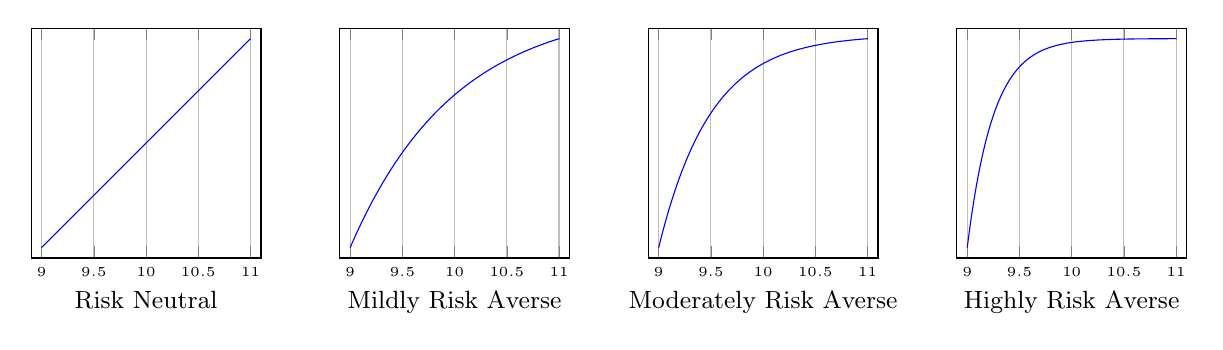
\begin{tikzpicture}
\begin{groupplot}[
    group style={
        group size=4 by 1,
        horizontal sep=1cm,
        vertical sep=1cm,
    },
    width=4.5cm,
    height=4.5cm,
    xmin=8.9, xmax=11.1, % Set the display range for x-axis
    ymin=8.9, ymax=11.1, % Set the display range for y-axis
    xtick={9,9.5,10,10.5,11},
    ytick=\empty, % Hide y-axis numbers
    xlabel style={at={(axis description cs:0.5,-0.1)},anchor=north, font=\small}, % Keep labels at small size
    xticklabel style={font=\tiny}, % Set x-axis numbers to be smaller
    grid=major,
    clip mode=individual % Limit the display to the specified range
]

% Risk Neutral (y = x)
\nextgroupplot[
    xlabel={Risk Neutral},
]
\addplot[blue, domain=9:11, samples=100] {x}; % Plot y = x only from 9 to 11

% Mildly Risk Averse (alpha = 1)
\nextgroupplot[
    xlabel={Mildly Risk Averse},
]
\addplot[blue, domain=9:11, samples=100] {9 + 2 * ((-exp(-1*x)) - (-exp(-1*9))) / ((-exp(-1*11)) - (-exp(-1*9)))};

% Moderately Risk Averse (alpha = 2)
\nextgroupplot[
    xlabel={Moderately Risk Averse},
]
\addplot[blue, domain=9:11, samples=100] {9 + 2 * ((-exp(-2*x)) - (-exp(-2*9))) / ((-exp(-2*11)) - (-exp(-2*9)))};

% Highly Risk Averse (alpha = 4)
\nextgroupplot[
    xlabel={Highly Risk Averse},
]
\addplot[blue, domain=9:11, samples=100] {9 + 2 * ((-exp(-4*x)) - (-exp(-4*9))) / ((-exp(-4*11)) - (-exp(-4*9)))};

\end{groupplot}
\end{tikzpicture}

\end{document}
